% Chapter 6

\chapter{Experiments} % Main chapter title

\label{Chapter6} % For referencing the chapter elsewhere, use \ref{Chapter1} 
In this chapter, we introduce the benchmark environments used to compute all the tests. We show the results obtained, the proposal for improvement, and a comparison between the model-free approach represented by the DDPG algorithm and the model-based approach represented by PlaNet.

\section{DeepMind Control Suite}
All the experiments are based on Deepmind Control Suite \cite{tassa2018deepmind}.
The control suite is a set of continuous control tasks that are built for benchmarking reinforcement learning agents. The main focus is on continuous control. The environments can provide a fully observable state (a feature vectors) and a partially observable state (a scene) frame. All the environments are written in Python and powered by the MuJoCo physics engine. A visual representation of the main environments available in the Deepmind control suite is shown below.


\begin{figure}[h]
\centering
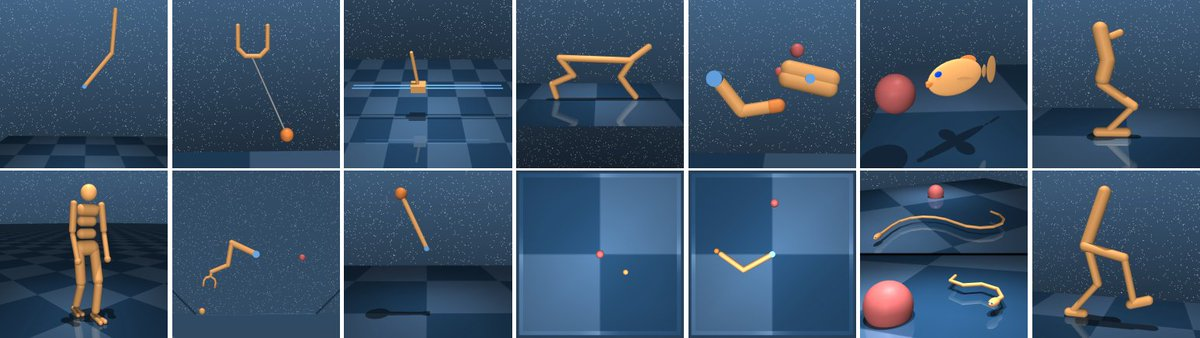
\includegraphics[width=1.0\textwidth]{pictures/dm_control}
                  \caption{. Top: Acrobot, Ball-in-cup, Cart-pole, Cheetah, Finger, Fish, Hopper.
Bottom: Humanoid, Manipulator, Pendulum, Point-mass, Reacher, Swimmer (6 and 15 links), Walker.}
            \end{figure}
The principal environment that we choose to experiment is the half-cheetah that is a very common choice. 

In this environment, the agent should move forward as quickly as possible with a cheetah like body that is constrained to the plane. The reward is linearly proportional to a maximum of $10_{\mathrm{m} / \mathrm{s}}$ i.e. $r(v)=\max (0, \min (v / 10,1))$.
A vector of 18 dimensions describes each state while the actions are represented with a vector of 6 dimensions.

In addition to this environment, we have chosen three more to test the consistency of the tests.

The other environments are:
\begin{itemize}
\item Cart-pole (task: swing-up): The classic cart-pole swing-up task. The agent must balance a pole attached to a cart by applying forces to the cart alone. The pole starts each episode hanging upside-down.

\item Walker (task: walk): Agent should move forward as quickly as possible with a bipedal walker constrained to the plane without falling or pitching the torso too far forward or backward.

\item Reacher: (mode: easy): The simple two-link planar reacher with a randomized target location. The reward is one when the end effector penetrates the target sphere.
\end{itemize}



\section{Model Free experiments }
We choose DDPG as a model-free algorithm for the experiments since it is compatible with environments with continuous action spaces. 
It also guarantees a good sample efficiency thanks to the buffer experience replay.

In this experiment we want to find out what level of performances a DDPG agent can reach with a million of steps.
We start from the original DDPG paper \cite{lillicrap2015continuous} but when it was released, the Deepmind control suite did not exist yet.
All the benchmarks in that paper, for the cheetah problem, are based on another suite provided by Open Ai called Gym.
Even if both the environments from Open Ai and Deepmind are based on the same physic engine (MuJoCo) and representing the same problem (the cheetah problem), they have significant differences that require a different set of parameters. 
All the parameters provided in the original paper are based on the Open Ai Gym version.

We addressed this problem in two phases.
At first, we precisely replicated the original paper model with the Open Ai Gym environment to be sure to have a solid implementation. 
We tried to retrain our model in the Deepmind Control Suite environment without the tuning process, without success. 
The DDPG algorithm proved to be very susceptible to the parameters. 
We tried another approach based on the Deepmind Control Suite paper in which the author explained how they trained the DDPG algorithm in their environments, and we are successfully reproduced their results.

In our implementation, we used Adam (\cite{kingma2014adam}) for learning the neural network parameters with a learning rate of $10^{-4}$ for both the actor and critic networks.
For the critic network, we included a $L_2$ weight decay of 0.002 and used a discount factor of $\gamma = 0.99$. 
We used both a soft update (with $\tau = 0.001$) and a hard update (every 100 steps) for the target networks. 
The activation function is the Relu for all the hidden layers and the Tanh for the actor final output layer.
After the activation, I apply batch normalization.
In the final layer (for both actor and critic networks) both the weight and bias are initialized from uniform distribution $\left[-3 \times 10^{-3}, 3 \times 10^{-3}\right]$.
The hidden layers instead are initialized from uniform distributions $\left[-\frac{1}{\sqrt{f}}, \frac{1}{\sqrt{f}}\right]$ where $f$ is the fan-in of the layer.
The actor-network is composed of 3 hidden layers with respectively [128,300,400] units.
Only for the actor-network, the gradients are clipped at [-1,1].
The critic-network is composed of two separate input layers (one for the action with 256 units and two for the state with 128,256 units). 
Then the two activations are summed together and passed to another 2 hidden layers with 300 and 400 units.
Lastly we used an Ornstein-Uhlenbeck process to produce the noise for the exploration. The parameters are: $\theta = 0.15$ and $\sigma = 0.3$.
We do not perform warm-up episodes to prefill the buffer before training.

The results of our experiments are shown below.
\begin{figure}[H]
\centering
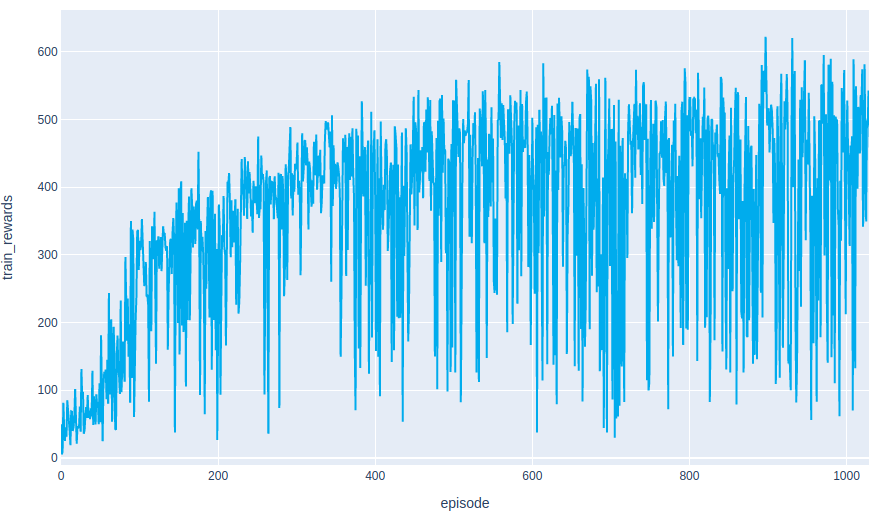
\includegraphics[width=1.\textwidth, height=.35\textheight]{pictures/ddpg_train_rew_with_feature_state}
\caption{ Results of the training of the DDPG algorithm on DeepMind Control Suite Ceetah environment.}
\end{figure}
Every episode corresponds to 1000 steps, and the training consists of 1 million steps.
During the training, at every action is added a gaussian noise.
To understand the real performance of the model, a test without noise is computed every 100 episodes.

\begin{figure}[H]
\centering
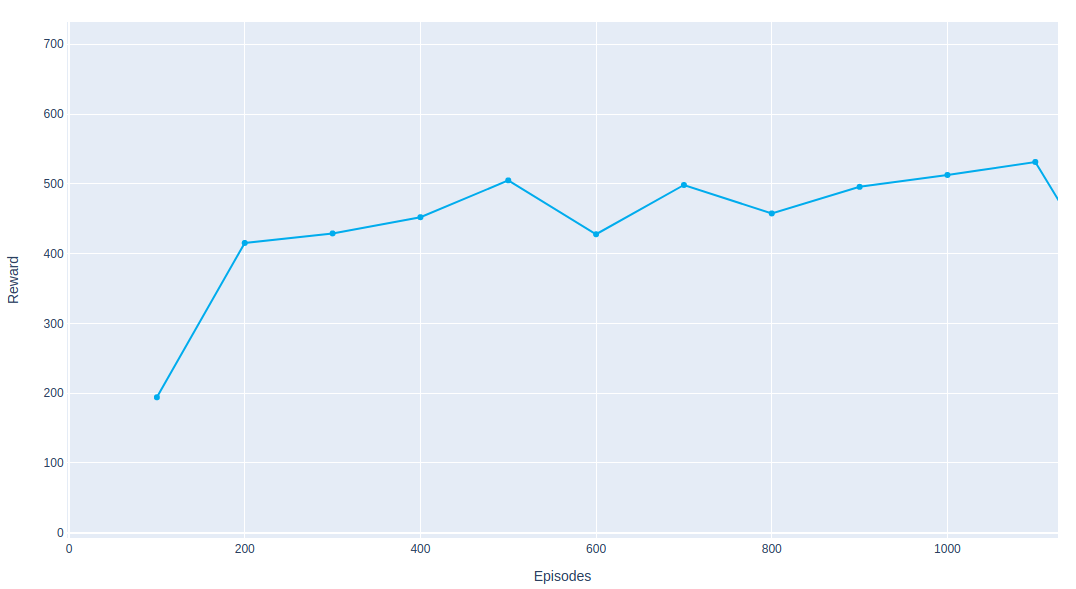
\includegraphics[width=.9\textwidth, height=.35\textheight]{pictures/ddpg_frame_as_input_test}
\caption{ Results of the test with the model trained with the DDPG algorithm from feature vectors.}
\end{figure}
This result is consistent with the performance published by the Deepmind Control Suite authors \cite{tassa2018deepmind}.

\begin{figure}[H]
\centering
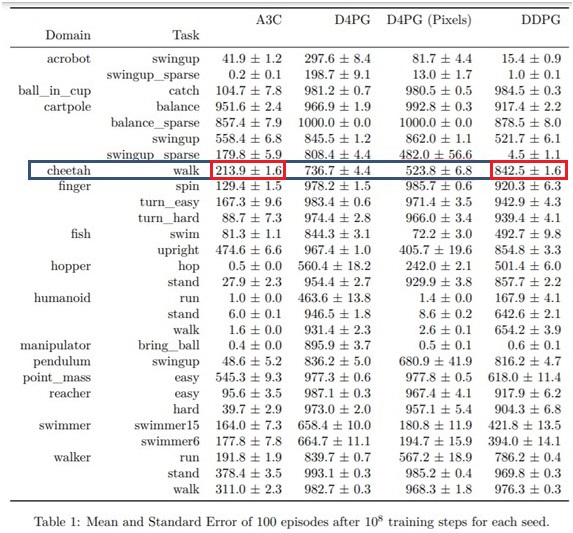
\includegraphics[width=.75 \textwidth, height=.45 \textheight]{pictures/dmcs_ddpg_vs_a3c}
\caption{ Result of the experiments from the Deepmind Control Suite team \cite{tassa2018deepmind}.}
\end{figure}

As we can see from the image above our implementation outperform the A3C algorithm and reach a cumulative reward value of 500 after $10^6$ steps that is compatible with the $812.5$ obtained from the research team after $10^8$ steps.


After our experiments, we can say that the DDPG algorithm is proved to be very sensitive to the hyperparameters.
We notice that some parameters like the initialization of the layers, the learning rate are more impact respect to the others.




\section{Model Free experiments from frames}
The use of the features vectors requires a human expert's intervention. This can be a limitation and also a source of error in the construction of the environment.

In this experiment, we want to find out if the DDPG algorithm is capable of solving this task directly from the raw pixels and in that case, how much the difficult of the problem increase.

With this new formulation, the observation provided does not correspond to the real markovian state of the MDP.
The authors of the Deepmind Control Suite doesn't use the DDPG algorithm to solve this problem but switched to an advanced version of the algorithm called  Distributed Distributional Deterministic Policy Gradients (\textbf{D4PG}).
They showed that this version of the algorithm after $10^8$ steps, is able to learn a policy also in this condition, but is not capable of achieving the same performances of the experiments with features vector as input. 

\begin{figure}[H]
\centering
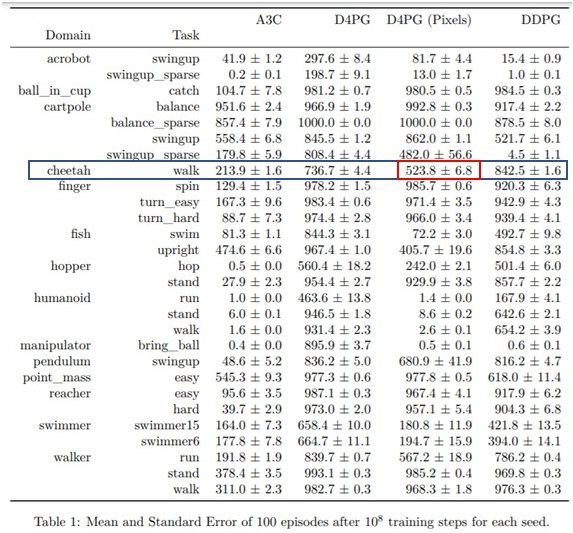
\includegraphics[width=.75 \textwidth, height=.45 \textheight]{pictures/dmcs_d4pg}
\caption{ Result of the Deepmind Control Suite team obtained with the D4PG algorithm\cite{tassa2018deepmind}.}
\end{figure}

We still tried to train a DDPG agent from raw pixels. 
As suggest in the original paper \cite{lillicrap2015continuous} we used the action repeats trick to enrich the information provided at each step. So at each step, the agent computes the same action 3 times. We have transformed the obtained 3 frames to grayscale, and we stacked them together the creating a new single input of 3 feature maps. The original version does not apply the grayscale conversion and provide an input of 9 feature maps. We notice anyway that this preprocessing step is very useful.
All the frames are downsampled to 64x64 pixels and normalized in a range between [0,1]. 
We added a new set of convolutional layers to the model to handle the frames high dimension.
We experimented with different approaches to network architecture.
Initially, I tried to create two convolutional networks, one for the actor and another for the critic but did not work well.
The best performance is obtained by weight-sharing of the convolutional network, as shown in the image below.

\begin{figure}[H]
\centering
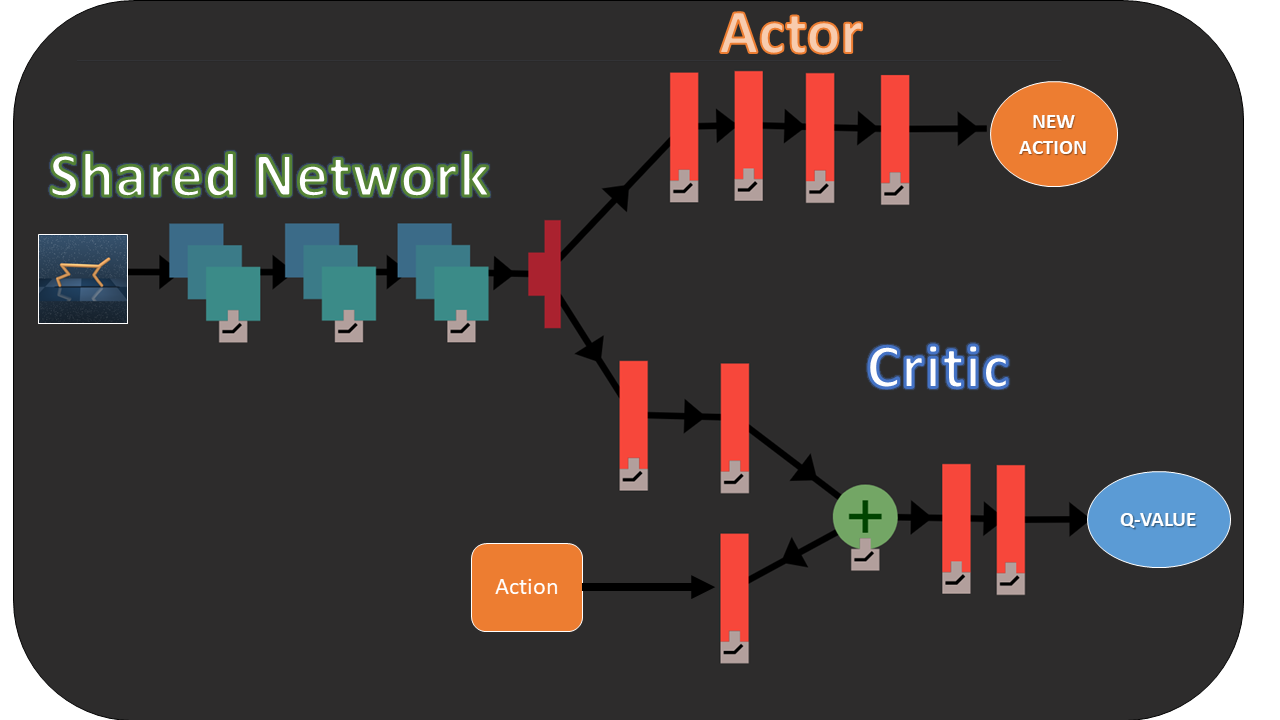
\includegraphics[width=1.\textwidth, height=.35\textheight]{pictures/ddpg_shared_net}
\caption{ Visual representation of the model architecture with the convolutional network shared between actor and critic.}
\end{figure}

Whenever the actor or the critic receives a frame as input, they call the shared convolutional network to encode the frames and return the corresponding features vector.
As suggested in \cite{tassa2018deepmind}, only the Critic network is allowed to update the shared network weights; in other words, the Actor gradients are truncated.
The shared network is composed of three layers, all with a kernel size of 3 x 3 with 32 channels (only the first layer with has also a stride of 2),  followed by two fully-connected layers with 200 and 50 neurons, with layer normalization.
All other parameters are the same as in the previous experiment, except the batch size is set to 256.

We stop the training after $10^6$ steps like all the other experiments. The results are shown below.

\begin{figure}[H]
\centering
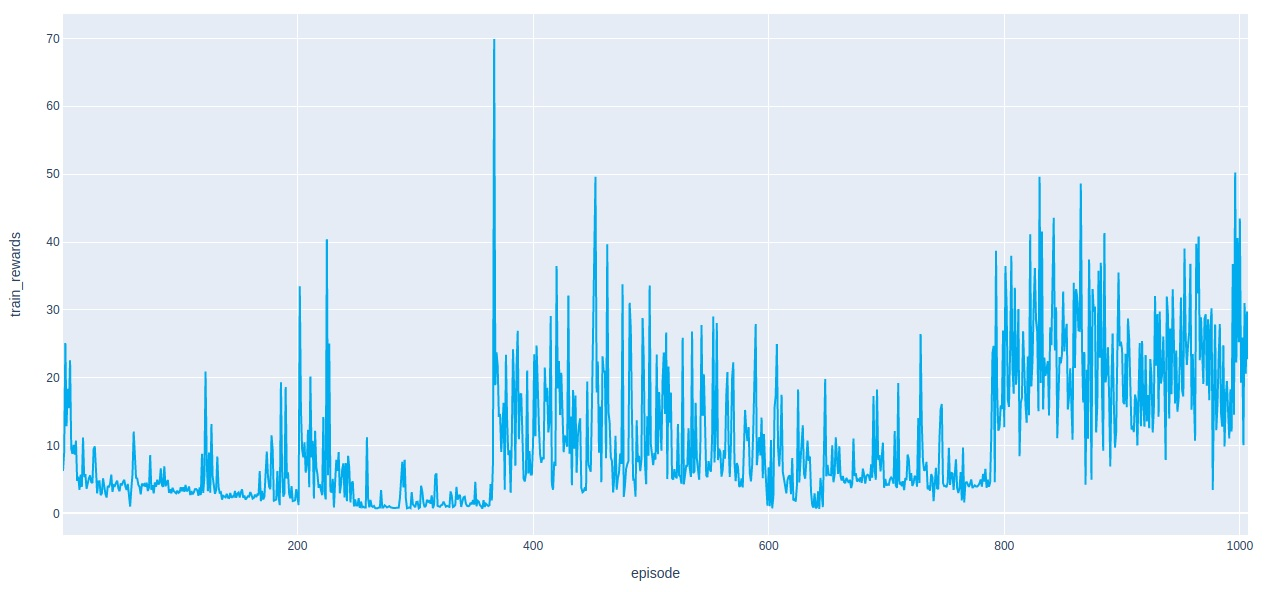
\includegraphics[width=1.\textwidth, height=.4\textheight]{pictures/ddpg_train_reward_with_frames_2}
\caption{ Result of training DDPG for the cheetah problem, after 1000 episodes using frames as input .}
\end{figure}

As we can see, after 1000 episodes (1 million steps), the agent is not able to reach significative performance. 
The training curve has risen slightly, indicating that full training would require several thousand more episodes.
Due to the limits of the computational budget is was not possible to train the network entirely.
%The test curve (obtained by using the same model at training time but without adding noise to the actions) confirms that after 1000 episodes, the training is just at most at the beginning phase, and the agent is not learning yet.

We suppose that the convolutional layers require a lot of transition before learning the useful pieces of information to capture from every image.
Until the convolutional layers are not trained, the policy can't learn.
We can clearly see how to learn from raw pixels is more complicated than learn from the features vector. 



\section{Model Based experiments }
The algorithm chosen for the model-based experiments is Planet.
We have not implemented it from scratch, but we build upon an open-source version available on \href{https://github.com/Kaixhin/PlaNet}{GitHub}.

We test the PlaNet algorithm on the same benchmark environment to see if this algorithm is able to solve in a million on steps the cheetah problem with raw pixels as input.

We do not operate tuning, so the parameters are the same as the open-source implementation, and we do not repeat them here.

\begin{figure}[H]
\centering
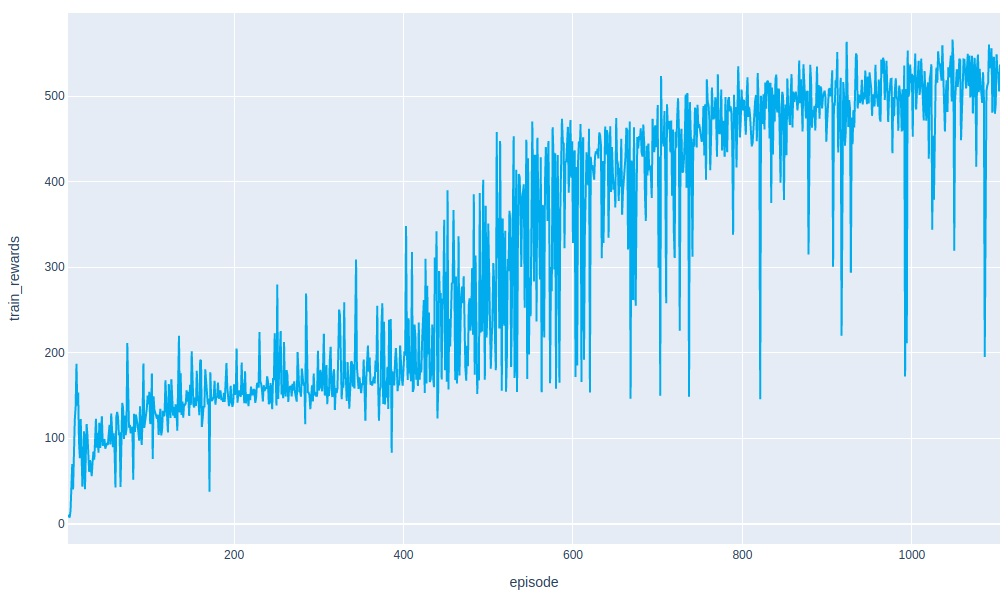
\includegraphics[width=1. \textwidth, height=.3\textheight]{pictures/train_resize}
\caption{ Performance obtained with the open source version of PlaNet at training time.}
\end{figure}

Like with the DDPG training, for every action, Gaussian noise is added, for this reason, there is a variance in the performance, but the training curve is monotonically increasing.

To find the real performance of the agent, we can see the test curve in which the same model is used without Gaussian noise.

\begin{figure}[H]
\centering
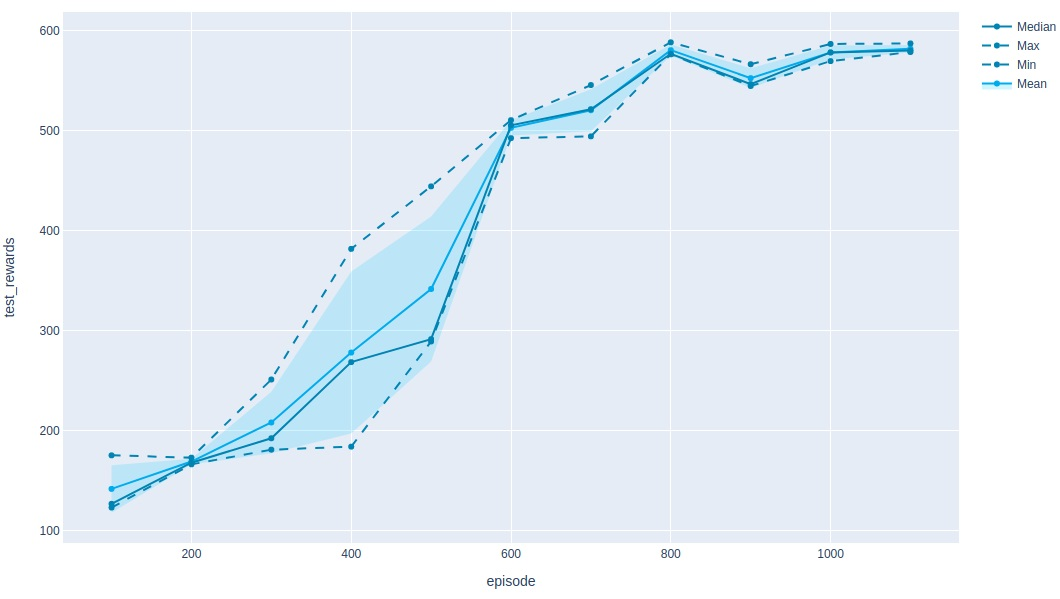
\includegraphics[width=1. \textwidth, height=.3\textheight]{pictures/test_resize}
\caption{ Performance obtained with the open source version of PlaNet at test time.}
\end{figure}

As we can see, after 1 million steps, the Planet agent is able to achieve a result of 578 rewards.


Beyond the final performances, it is interesting to deeply analyze the model predictions and the ability to generate predicted frames.
So in this experiment, we focus on the visual component of the prediction model.

We only provided the first frame to the model, and it predicted all the rest without receiving any further information beyond the actions performed at each step.

Both the observations and the predicted frames are resized to 64 x 64 pixels in order to reduce the computational cost. 

\begin{figure}[H]
\centering
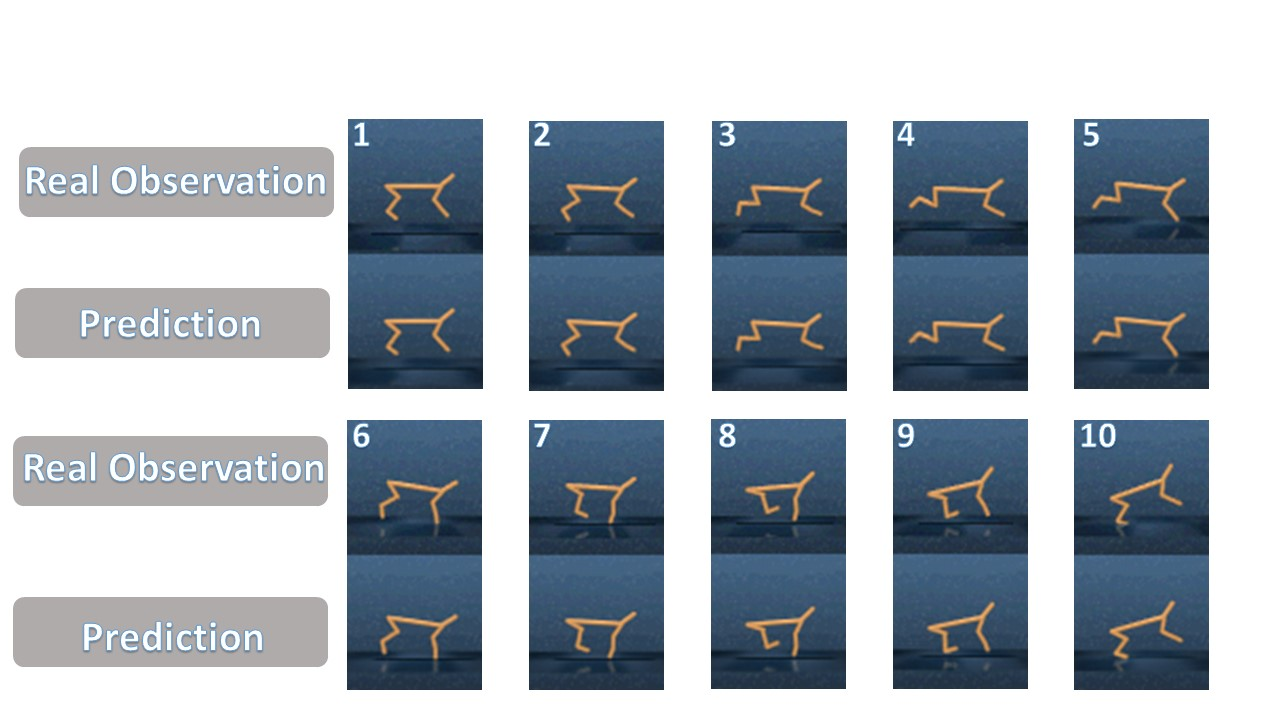
\includegraphics[width=1. \textwidth, height=.35\textheight]{pictures/dump_plan_init}
\caption{ Comparison between the first 10 real observations (the top frame) and the 10 predictions (the bottom frame).}
\end{figure}

As we can see from the image above, the model is able to predict all the first 10 steps correctly, but it is hard to keep the memory of the past experience for a long time, so as the predictions go on, the errors pile up.
Initially, these errors are barely perceptible. For this reason, we have extended the planning horizon up to 20 steps reaching the point where these errors are easily visible.

\begin{figure}[H]
\centering
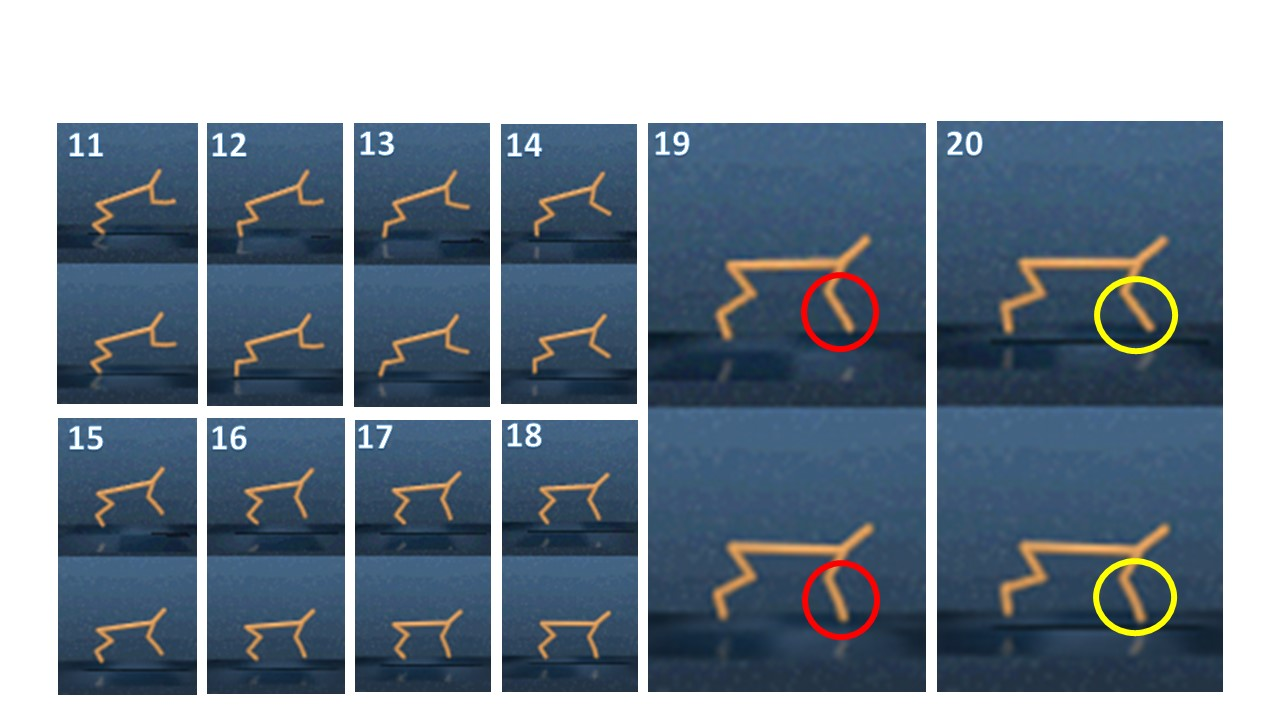
\includegraphics[width=1. \textwidth, height=.35\textheight]{pictures/dump_plan_finish}
\caption{ We can start to see discrepancies as the predictions goes on.}
\end{figure}

In order to make this comparison more clearly, we calculate the mean squared error (MSE) of each frames and we plot the pixels difference over the 20 planned steps.

\begin{figure}[H]
\centering
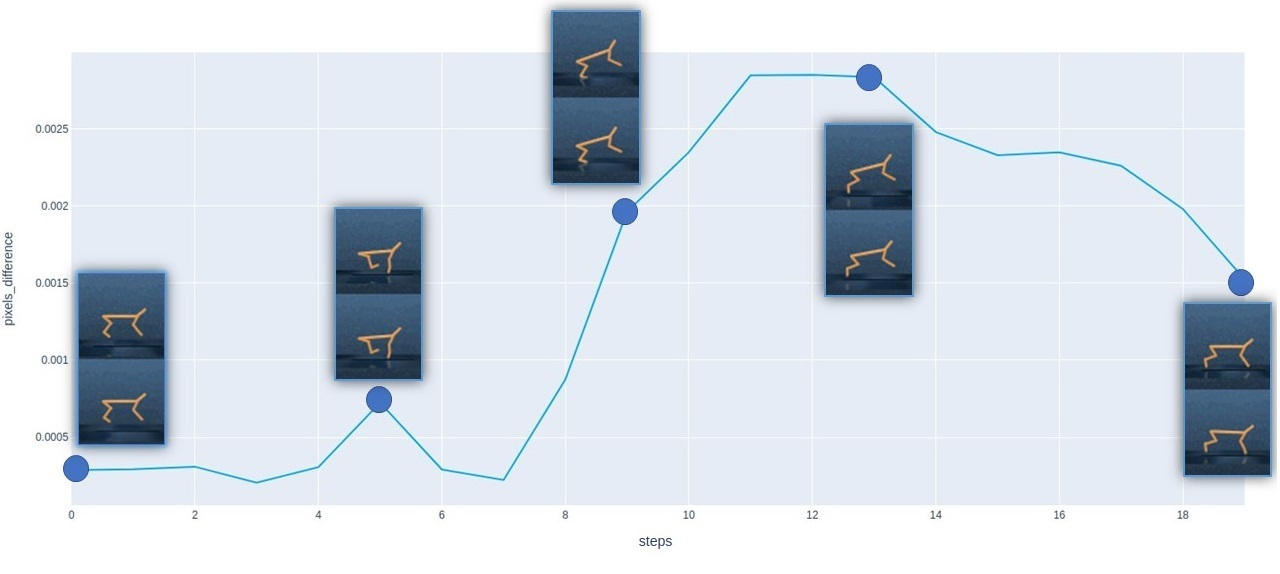
\includegraphics[width=1. \textwidth, height=.35\textheight]{pictures/pixels_difference}
\caption{The mean squared error of the real and predicted frames over 20 steps.}
\end{figure}
This is not a problem for the planning algorithm since the model predict only for a short horizon. In particular the authors of PlaNet has chosen a planning horizon of 12 steps.

We have also produced a heatmap to highlight the area in which the model produce the most errors.

\begin{figure}[H]
\centering
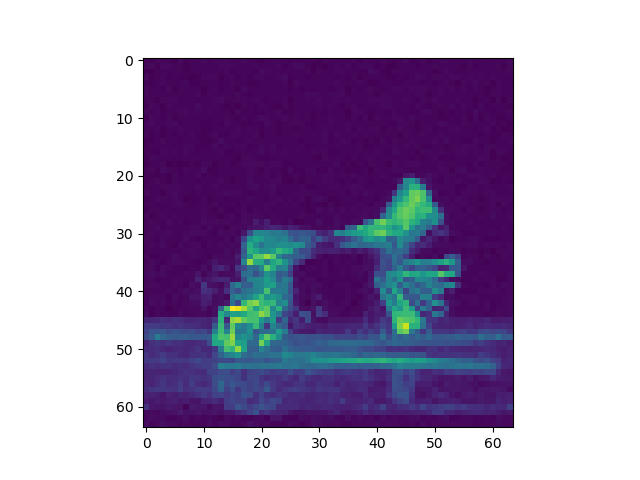
\includegraphics[width=1. \textwidth, height=.45\textheight]{pictures/heatmap}
\caption{The heatmap highlight the area of all the predicted frames where the model has made the greatest errors.}
\end{figure}
As we could expect the heatmap show that the model make more error in the area of the in the hind and front legs of the cheetah and in the zone of the head.

We also tested the reward predictions. The plot below show how close are the predictions of the fully trained model and the effective received reward for an entire episode.

\begin{figure}[H]
\centering
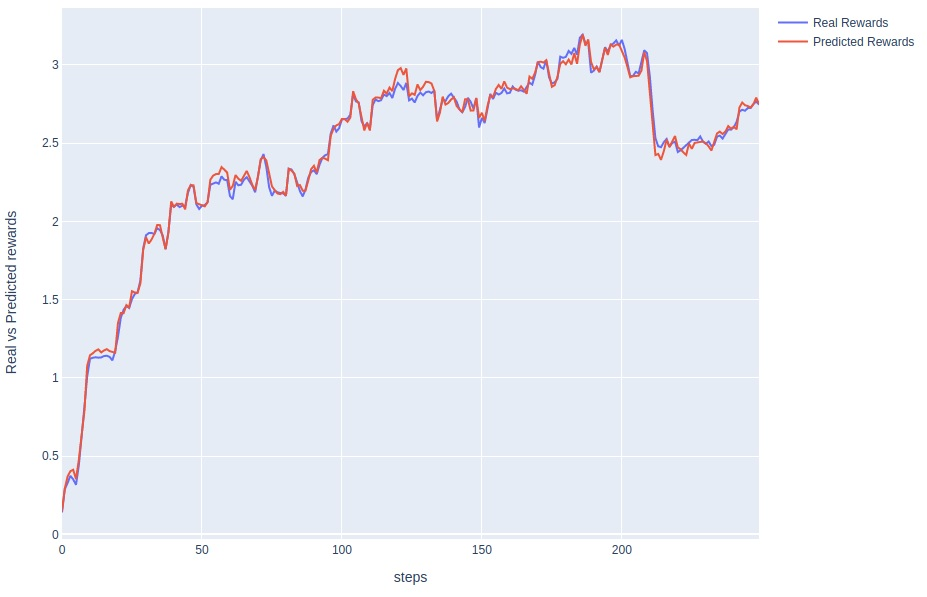
\includegraphics[width=1. \textwidth, height=.4\textheight]{pictures/rew_vs_pred_rew}
\caption{ Comparison between the reward model predictions and the effective reward obtained.}
\end{figure}


\section{Experiments with PlaNet}

In this section we investigate the chance to improve the performance of the open-source version of PlaNet. We tried three different ways.

The first try is about the preprocessing phase of each frame steps.
At each steps, the generated frame is preprocessed before being used as input to the model. In particular, operation of resizing is applied by the cv2 library using the INTER LINEAR algorithm.
Exploring the DeepMind Control Suite code, we saw that this process could be avoided indicating directly to the camera the size of the frame to be rendered with the command:
\textit{\texttt{self.\textunderscore env.physics.render(height=64, width=64, camera\textunderscore id=0)}}.
We found that also the original implementation uses a resize method instead of native render in low dimensions. In particular they use the \textit{"skimage.transform.resize"} method as you can see in \href{https://github.com/google-research/planet/blob/master/planet/control/wrappers.py}{their implementation}. 

We can see how changing this single one line of code has a huge positive impact on the final performance.

\begin{figure}[H]
\centering
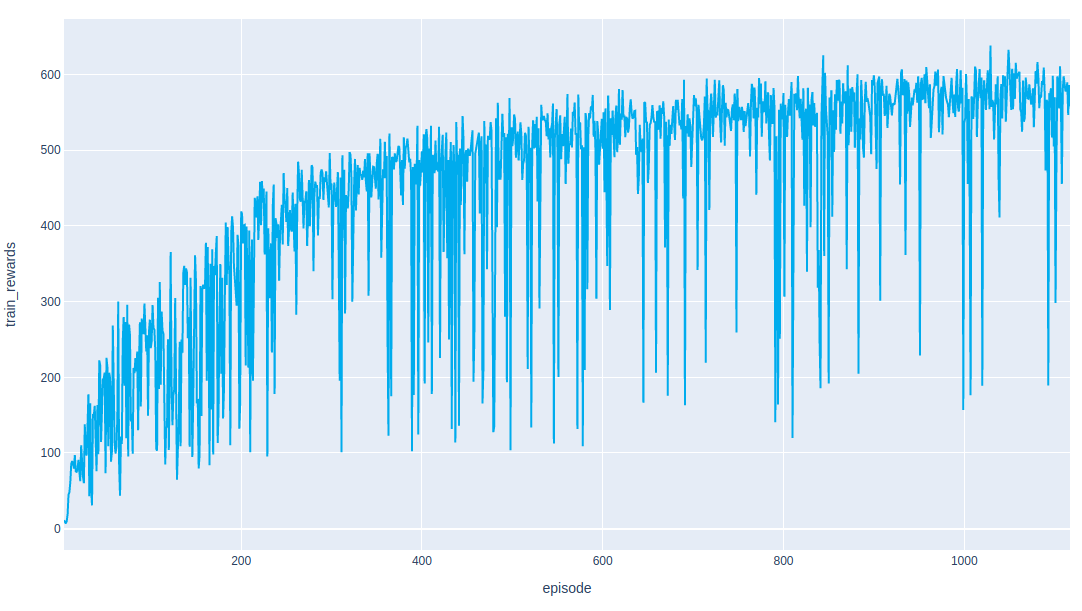
\includegraphics[width=1. \textwidth, height=.3\textheight]{pictures/train_planet_puro}
\caption{ Performance obtained at training time without resize the frames.}
\end{figure}

\begin{figure}[H]
\centering
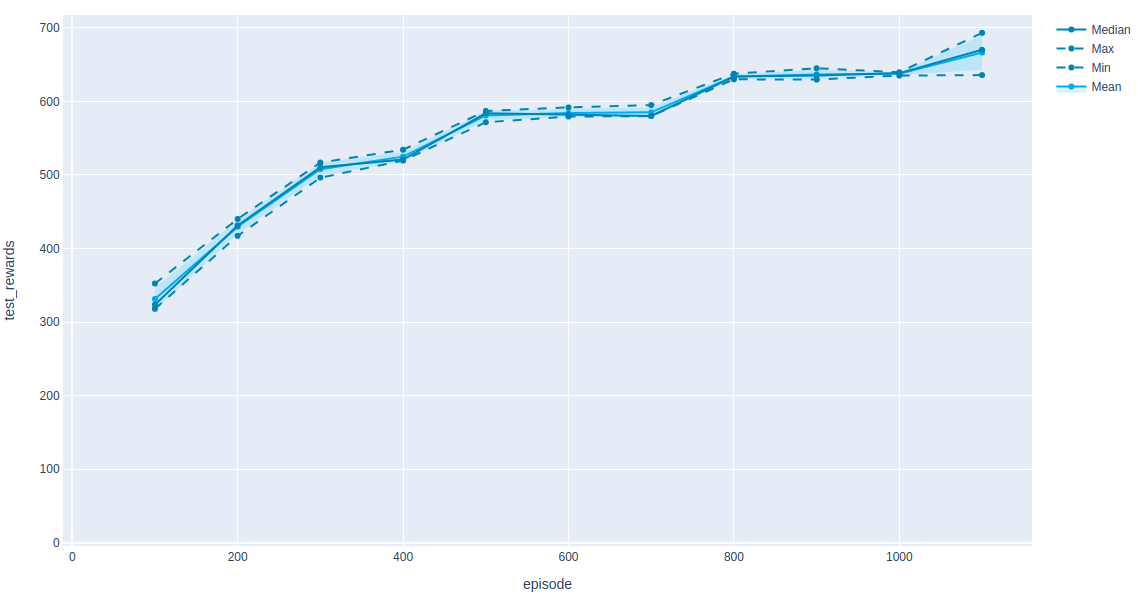
\includegraphics[width=1. \textwidth, height=.3\textheight]{pictures/test_planet_puro}
\caption{ Performance obtained at test time without resize the frame.}
\end{figure}

\begin{figure}[H]
\centering
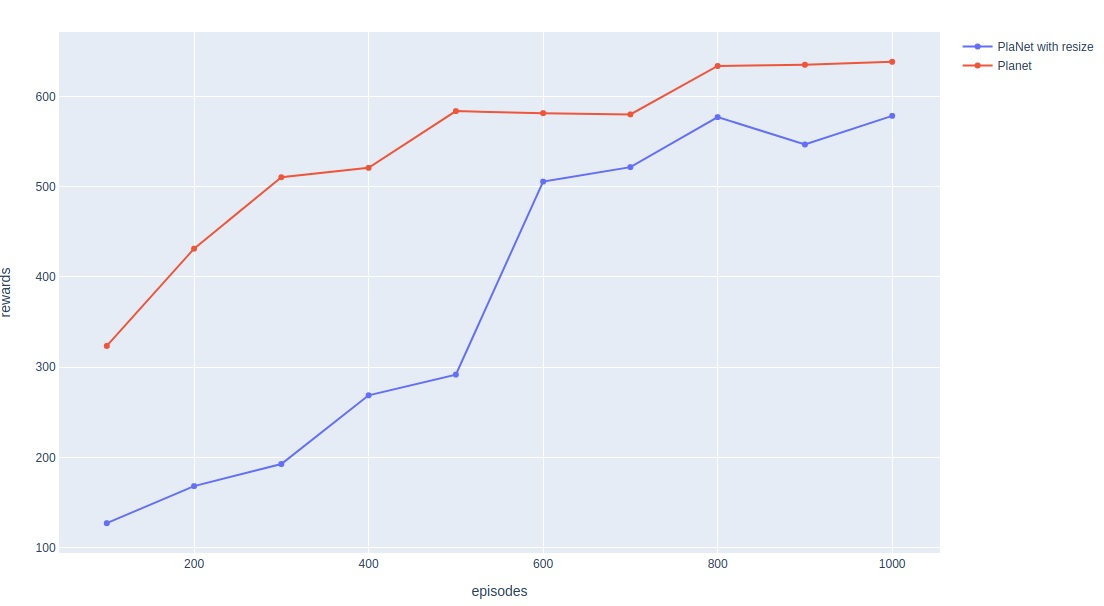
\includegraphics[width=1. \textwidth, height=.3\textheight]{pictures/resize_vs_pure}
\caption{ Comparison between the performance of PlaNet with and without the frames resizing.}
\end{figure}

We think that this improvement is due to the fact that some information is lost when the algorithm of resizing are applied in the preprocessing phase.
\\
A second experiment is based on the idea of enriching the information at each step with the obtained reward, in addition to the current frame. During the experiments, we notice that when the model is not fully trained can happen that it keeps doing the same action believing to collect rewards. Indeed what really happening is that the agent keeps predicting a reward when in the real environment, it doesn't receive any good feedback.
After some training iterations, the agent fits better the environment dynamics, and the problem disappears. So the idea is to explicitly provide also the received reward so the agent can use it to recognize, at inference time, that it's predictions are not consistent with what is really happening. So, we modify the model by concatenating the encoded current observation with the previous reward.

\begin{figure}[H]
\centering
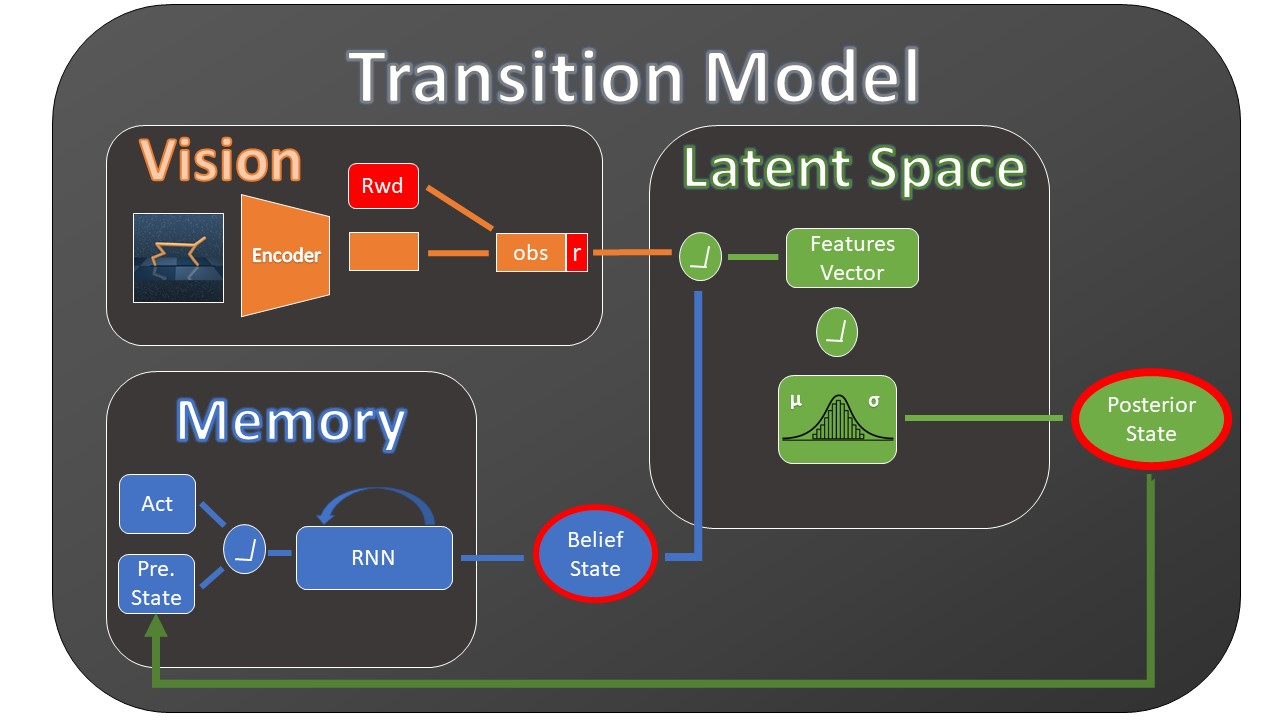
\includegraphics[width=1. \textwidth, height=.35\textheight]{pictures/planet_pred_as_rew}
\caption{ Concatenating the reward to the current observation.}
\end{figure}
The result of training seems to be not so promising. The training curve has more variance and does not overcome the previous version. 

\begin{figure}[H]
\centering
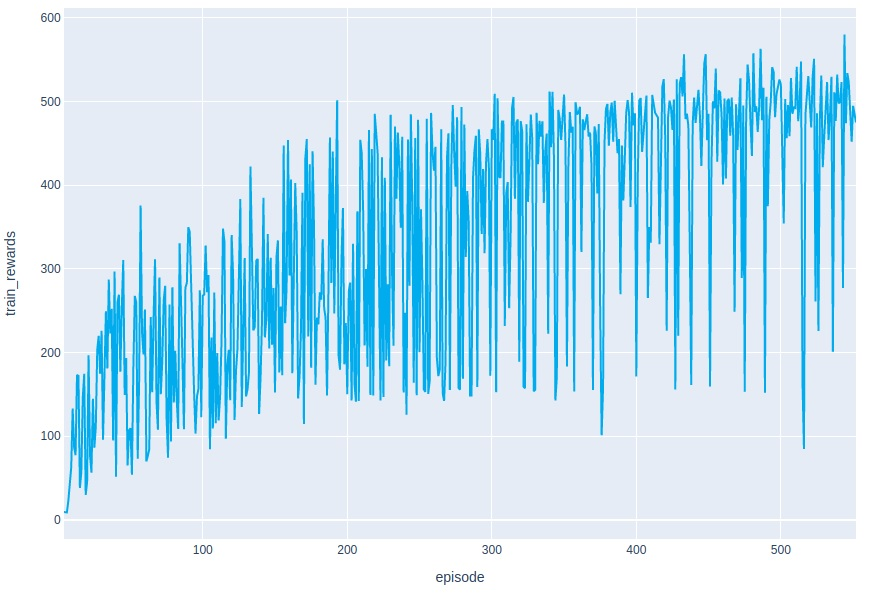
\includegraphics[width=1. \textwidth, height=.4\textheight]{pictures/planet_train_rew_as_state}
\caption{ Training curve of Planet model with reward as input.}
\end{figure}
The test curve confirms that this model is worse than the original. 

\begin{figure}[H]
\centering
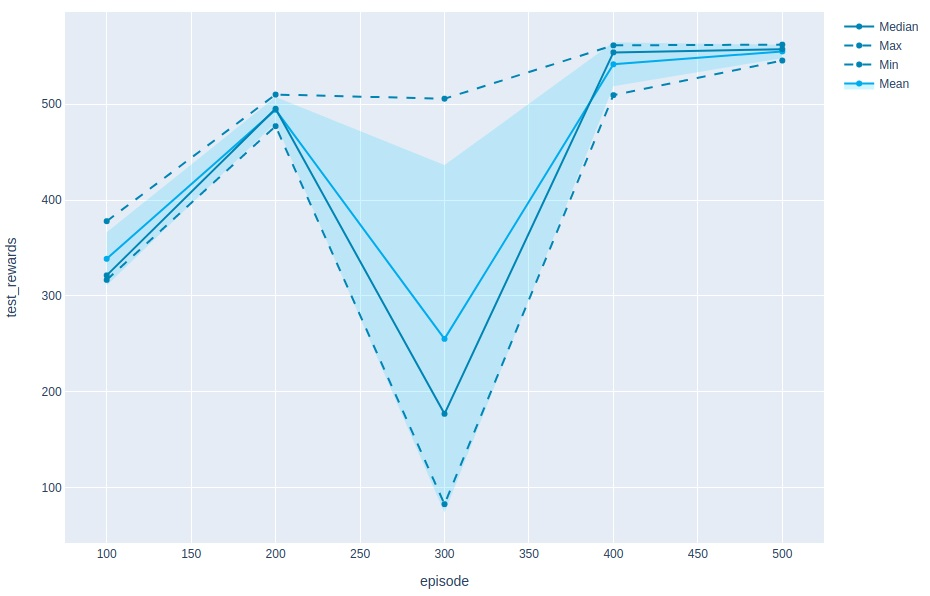
\includegraphics[width=1. \textwidth, height=.35\textheight]{pictures/planet_test_rew_as_state}
\caption{ The test curve is more unstable and achieve less cumulative reward than the original model. }
\end{figure}

After 500 iterations, we saw that the model is not outperforming the original version and we stop the experiment.

\begin{figure}[H]
\centering
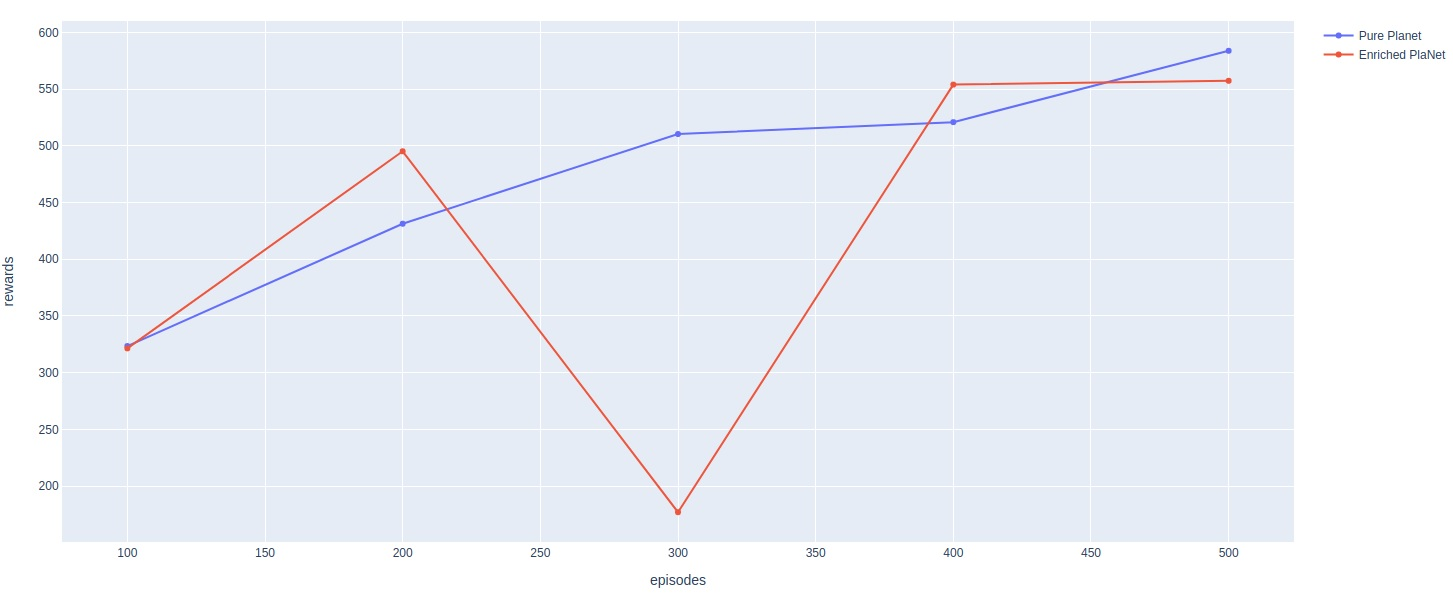
\includegraphics[width=1. \textwidth, height=.35\textheight]{pictures/rew_as_state_vs_pure_planet}
\caption{ The test curve is more unstable and achieve less cumulative reward than the original model. }
\end{figure}
We tried to add the reward information to other components of the model (e.g., in the memory module or directly in the reward module), but none of these tests worked and the presented version is the one that has given the best results. 
\\
The last idea is to add regularizer to improve the model predictions.
One of the main problems of using a planner in a model that is just an approximation of the real environment dynamics, is that the planner will exploit the learned model models inaccuracies. So, in the areas in which the model is uncertain, the predictions tend to be too optimistic and lead the planner to sub-optimal actions. 
We plot a comparison of the predicted and the rel reward obtained during the initial training episodes. From the image below we can see how initially the predictions tends to be too optimistic, and the provided plan fail to reach the expectations obtaining a low reward.

\begin{figure}[H]
\label{fig:original_rew_vs_pred}
\centering
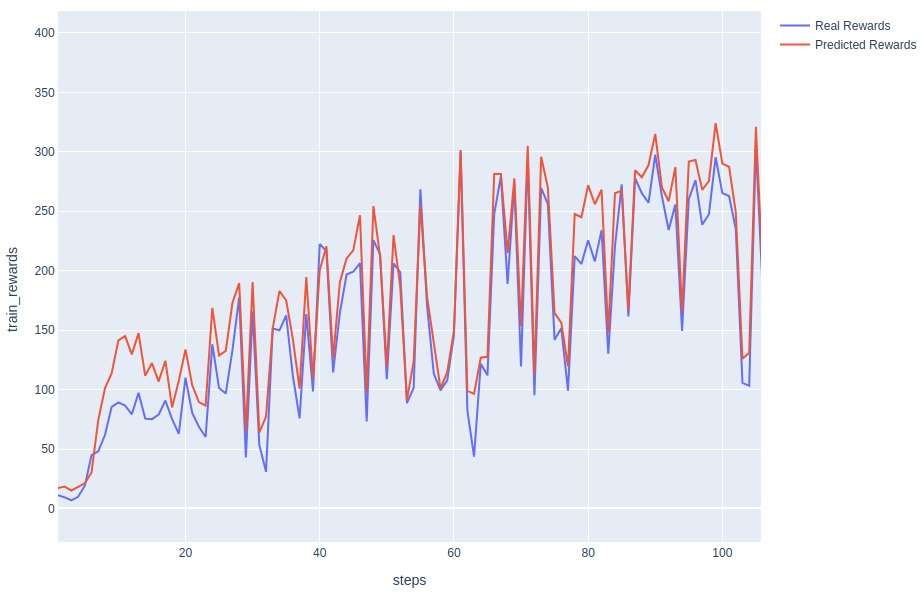
\includegraphics[width=1. \textwidth, height=.35\textheight]{pictures/original_pred_vs_real_rew}
\caption{ Comparison between the expected rewards predictions and the actual rewards obtained from the first 100 training episodes. }
\end{figure}
This problem is more severe in the early stages and less in later episodes when the agent has collected more data. Indeed, the more the agent interacts with the environment, the more data it collects, the more the predictions are precise. We are investigating a method to reduce this prediction gap just from the first episodes.

In their research, Rinu Boney et all \cite{boney2019regularizing} tries to alleviate this problem by penalizing the optimizer from considering trajectories that are outside the experience replay buffer ( that contains all the past experiences).
We call this new metric: \textbf{familiarity of the trajectories}.
So the planning objective is to maximize the rewards and also the familiarity of the plan respect to the data, with a new parameter $\alpha$ that modulates the weight between both costs.

$a_{t}^{*}, \ldots, a_{t+H}^{*}=\underset{a_{t}, \ldots, a_{t+H}}{\operatorname{argmax}} \sum_{\tau=t}^{t+H} r\left(s_{\tau}, a_{\tau}\right)+\alpha \log p\left(s_{t}, a_{t}, s_{t+1}, \ldots, s_{t+H}, a_{t+H}, s_{t+H+1}\right)$

Where $p(o_t, a_t, . . . , o_{t+H}, a_{t+H})$ is the probability of observing a given trajectory in the past experience.
They approximate the joint probability
of the whole trajectory as a sum of joint probabilities of each transition in the trajectory

$a_{t}^{*}, \ldots, a_{t+H}^{*}=\underset{a_{t}, \ldots, a_{t+H}}{\operatorname{argmax}} \sum_{\tau=t}^{t+H}\left[r\left(s_{\tau}, a_{\tau}\right)+\alpha \log p\left(s_{\tau}, a_{\tau}, s_{\tau+1}\right)\right]$

To calculate $\log p\left(s_{\tau}, a_{\tau}, s_{\tau+1}\right)$ they uses a denoising autoencoder (DAE).
DAE does not build an explicit probabilistic model $p\left(s_{\tau}, a_{\tau}, s_{\tau+1}\right)$ but learns to approximate the derivative of the log probability density.
To be more specific the theory of denoising states that, for zero-mean Gaussian corruption, the optima denoising function $g(\tilde{x})$ is given by:
$g(\tilde{x})=\tilde{x}+\sigma_{n}^{2} \frac{\partial}{\partial \tilde{x}} \log p(\tilde{x})$
where $\tilde{x}$  is the corrupted input, $p(\tilde{x})$ is the probability density function for $\tilde{x}$, $\sigma_n$ is the standard deviation of the Gaussian corruption.
So given the corrupted input $\tilde{x}$ and a fully trained DAE $g(\tilde{x})$, we can derive the gradient of the log-probability of the data distribution convolved with a Gaussian distribution:
$\frac{\partial}{\partial \tilde{x}} \log p(\tilde{x}) \propto g(x)-x$. 
They use $\frac{\partial}{\partial \tilde{x}} \log p(\tilde{x}) $ instead of $\frac{\partial}{\partial \tilde{x}} \log p(x) $ assuming $\frac{\partial}{\partial \tilde{x}} \log p(\tilde{x}) \approx \frac{\partial}{\partial x} \log p(x)$.
\\
For the experiments, they used an environment with low dimensional input (features state) and so with another model based algorithm, called PETS \cite{chua2018deep}. 
We initially try to replicate their solution, but the difference between the two models and the overload due to the processing of the image (they worked only with features vectors, not with frames) make the model so slow to be useless. 
For this reason, we use the same idea, but we implement it differently. We work directly with the prediction model and not with the planned.  Another fundamental difference is that we work at training time and not at inference time.
The PlaNet prediction model does not produce directly a new observation but works only in a latent space. So it makes no sense to train DAE with the observations collected in the dataset. Instead, we train the DAE directly in latent space also at training time.
The second difference is about the input dimension.
We feed the DAE with the entire plan at each step, so we train it by concatenating all the transitions according to the planning horizon parameter.
We experiments to different ways to concatenate transitions:
\begin{enumerate}
\item Concatenation of triplets: every transition is composed by 3 elements: $(s_t,a_t,s_{t+1})$. But in the final concatenation, all the elements placed at the extremes will be repeated: $[ (s_0,a_0,s_1) , (s_1,a_1,s_2) ... (s_{10},a_{10},s_{11}),  (s_{11},a_{11},s_{12}) ]$
\item Concatenation as chain: we remove the repetitions: $[ (s_0,a_0,s_1,a_2,s_2 ... s_{10},a_{10},s_{11},a_{11},s_{12}) ]$
\end{enumerate}

\begin{figure}[H]
\centering
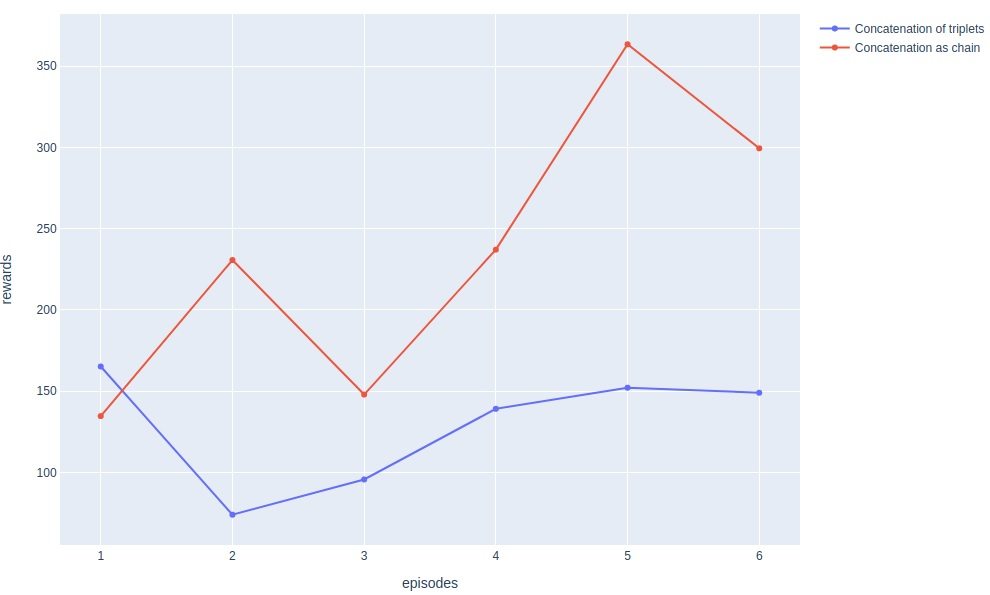
\includegraphics[width=.90 \textwidth, height=.25\textheight]{pictures/comparison_chain_vs_tripl}
\caption{ Comparison between the two strategies of input shape for the regularizer. }
\end{figure}

The final model architecture consists of one single linear layer with 600 units and a gaussian noise of zero mean and a standard deviation of 0.3.
The input dimension is the sum of the belief state size, the posterior state size, and the size of the actions multiplied for the planning horizon.
As we expected, the regularizer's effect is to improve the model predictions immediately and allow the model to increment the sample efficiently just from the initial episodes.


\begin{figure}[H]
\centering
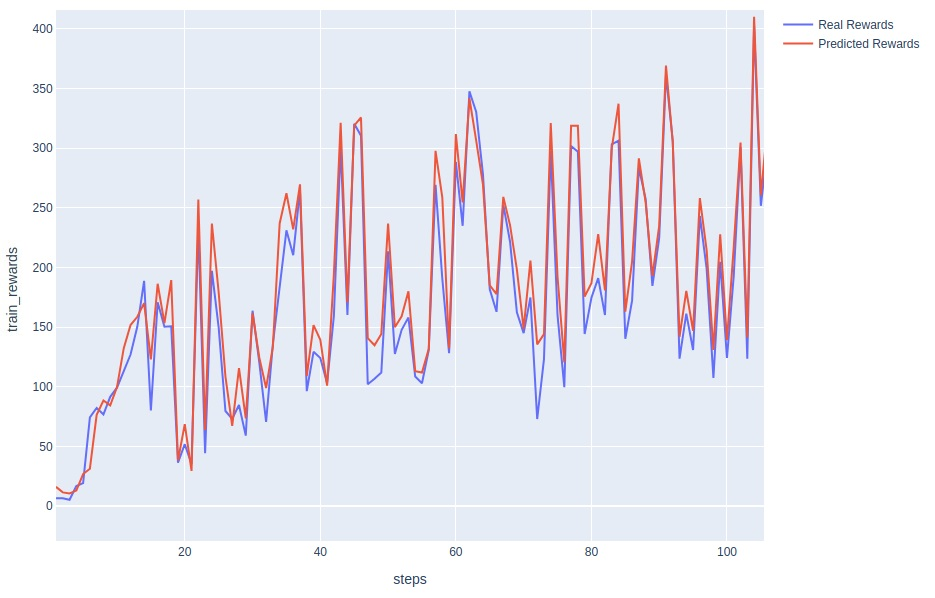
\includegraphics[width=1. \textwidth, height=.35\textheight]{pictures/reg_pred_vs_real_rew}
\caption{ Comparison between the expected rewards predictions and the actual rewards obtained from the first 100 training episodes with regularizer. }
\end{figure}
We can see from the image above that the reward's predictions start immediately to match with the real reward when the regularizer is activated.  
To make more clear the comparison between the prediction of the model with and without the regularizer, we created a new plot. 
In this plot we indicate the difference between the predicted reward and the obtained one over the episodes of the training. 
We can clearly see that the prediction error of the regularized model, represented with the blue line, is clearly lower in the initial episodes and that after some episodes the two values starts to converge.

\begin{figure}[H]
\centering
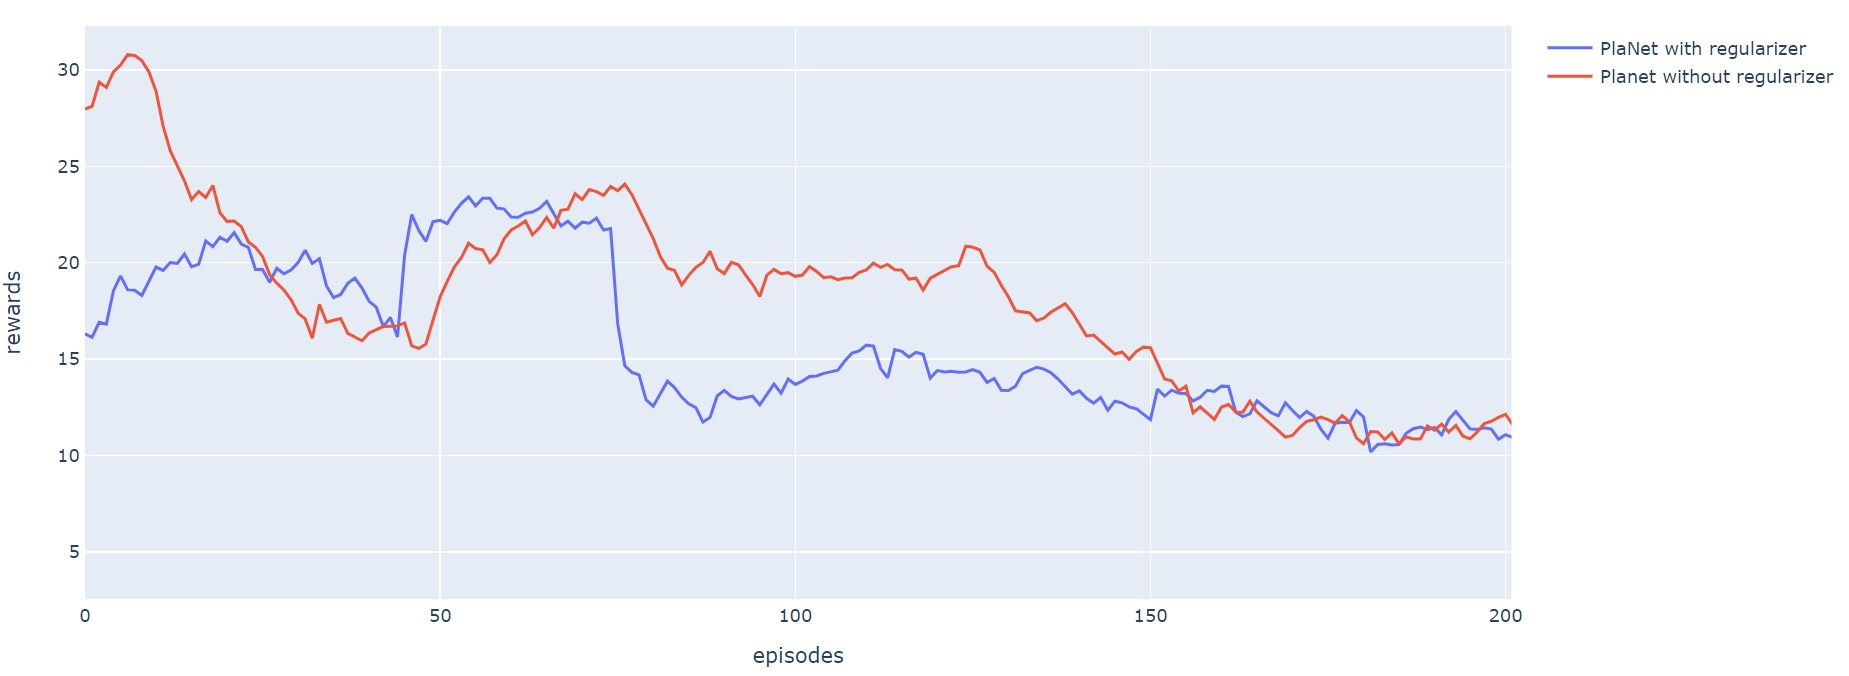
\includegraphics[width=1. \textwidth, height=.25\textheight]{pictures/plot_ass_diff}
\caption{ The absolute reward prediction error. The moving average technique is applied with a window of 30. }
\end{figure}

To be more clear we also calculate the relative error that remain consistent with the results above.

\begin{figure}[H]
\centering
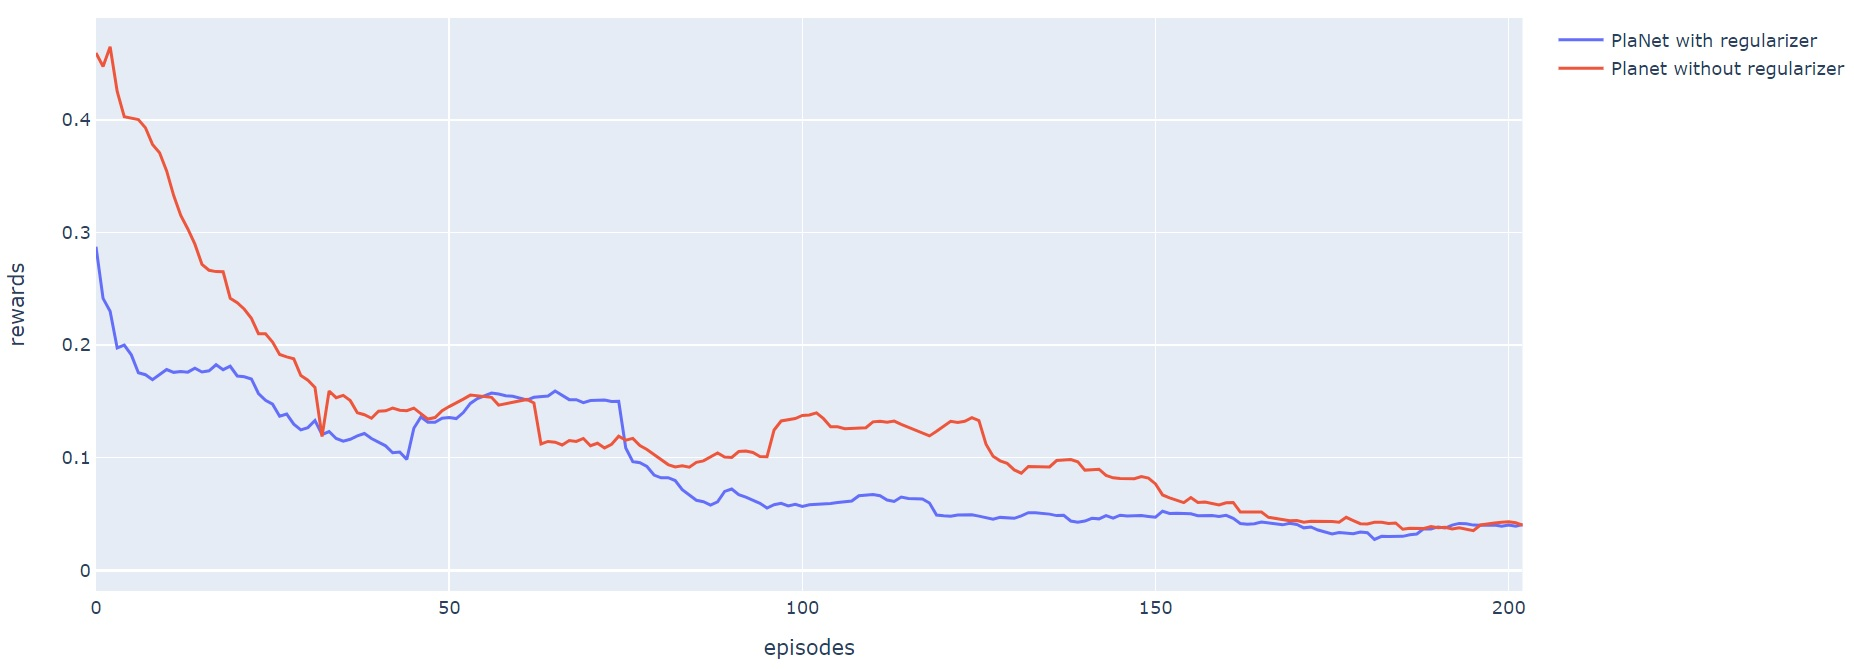
\includegraphics[width=1. \textwidth, height=.25\textheight]{pictures/plot_rel_diff}
\caption{ The relative reward prediction error. The moving average technique is applied with a window of 30. }
\end{figure}

This improvement allows the model to accumulate more rewards just in the initial episodes. This can be very useful where it is not possible to produce a huge amount of data.
\begin{figure}[H]
\centering
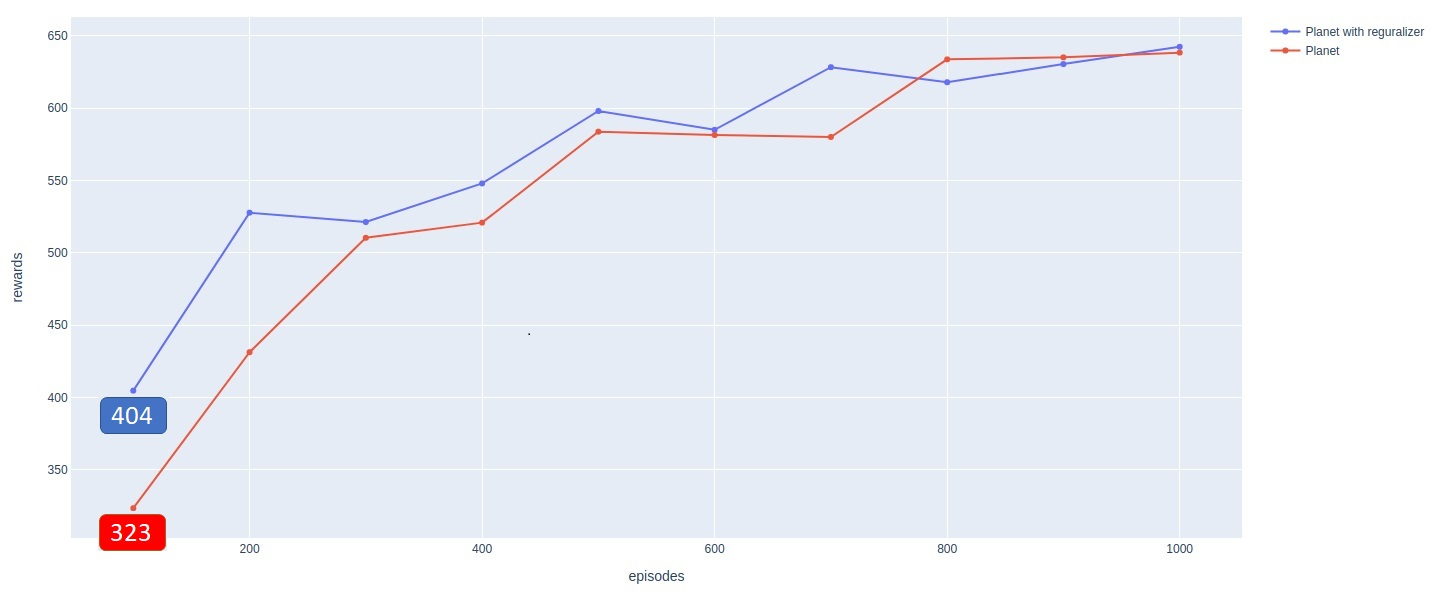
\includegraphics[width=1. \textwidth, height=.25\textheight]{pictures/full_reg_vs_original}
\caption{ Comparison between the full trained model with and without the regularizer.  }
\end{figure}

According to the research of Rinu Boney et all \cite{boney2019regularizing}, the improvement of the regularizer decrease during the training, but in our case, the performance of the original model does not surpass the performance of the model with regularized. 
%As suggested by the Rinu Boney et al. paper, "This result is evidence of the importance of exploration: the DAE regularization essentially penalizes exploration, which can harm asymptotic performance in complex environments."
We think that after a certain number of iterations, the model has accumulated enough knowledge about the environment to do without the regularizer. As proof of this, we point out that to achieve these results, we have to decrease the impact of the regularizer during training. From episode 750, we deactivate it entirely.
We observed an improvement, that needs to be validated with other experiments on other environments.


\section{Comparisons}
Now it's time to compare the model-based and the model-free approach. 

We specify that for this final comparison we use the DDPG result obtained with the model trained from the features vectors, while the PlaNet results are obtained with a model trained via raw pixels.

Despite the difference in the input complexity, the model-based approach achieves better results. In particular, in the initial phase, when the model has less sample and the regularizer influence is more intense.

\begin{figure}[H]
\centering
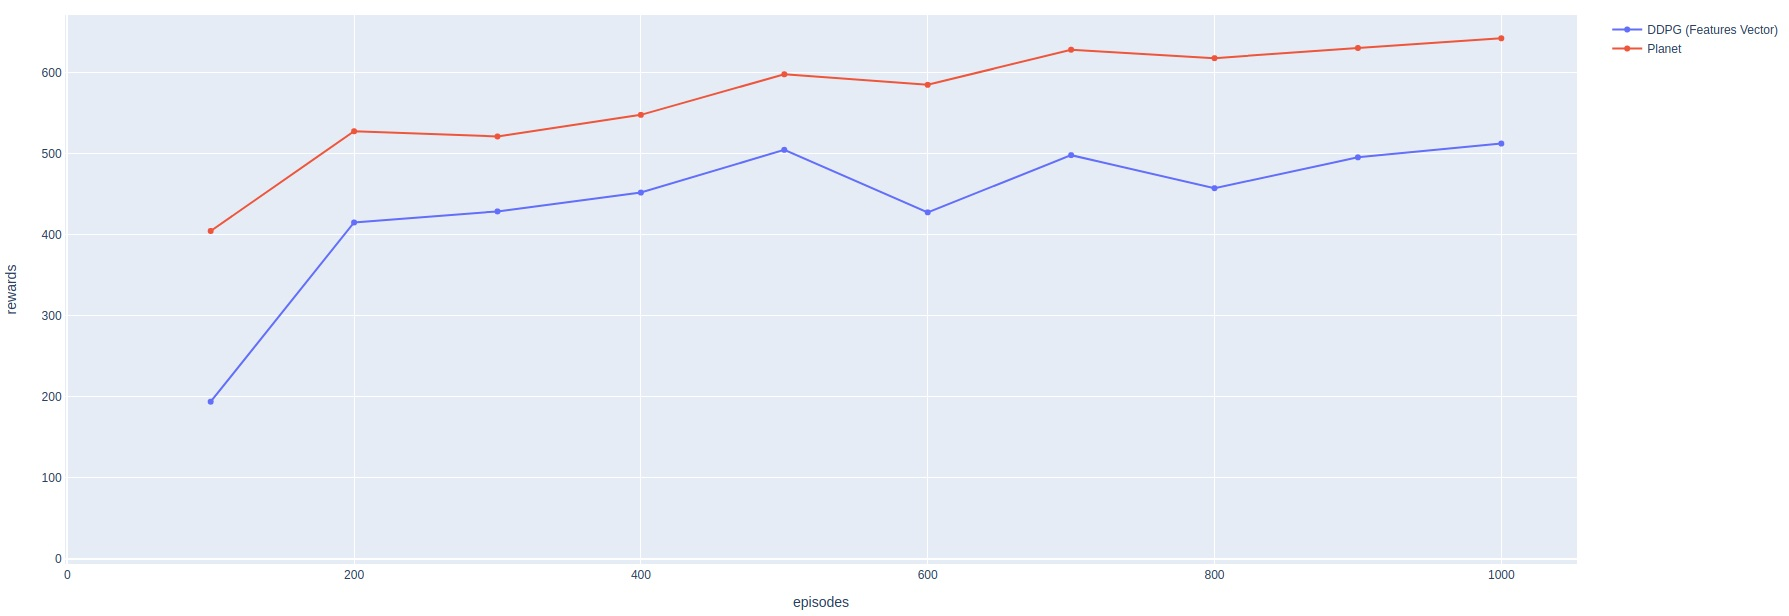
\includegraphics[width=1 \textwidth, height=.25\textheight]{pictures/ceetah_planet_vs_ddpg}
\caption{ Comparison between the performance of PlaNet (trained from frames) and DDPG (trained fro features vectors) for the Ceetah environment.  }
\end{figure}

We also tried other different environments, and we saw that PlaNet roughly maintain the advantage over DDPG. 
We specify that for these other environments, we do not use the regularizer.

\begin{figure}[H]
\centering
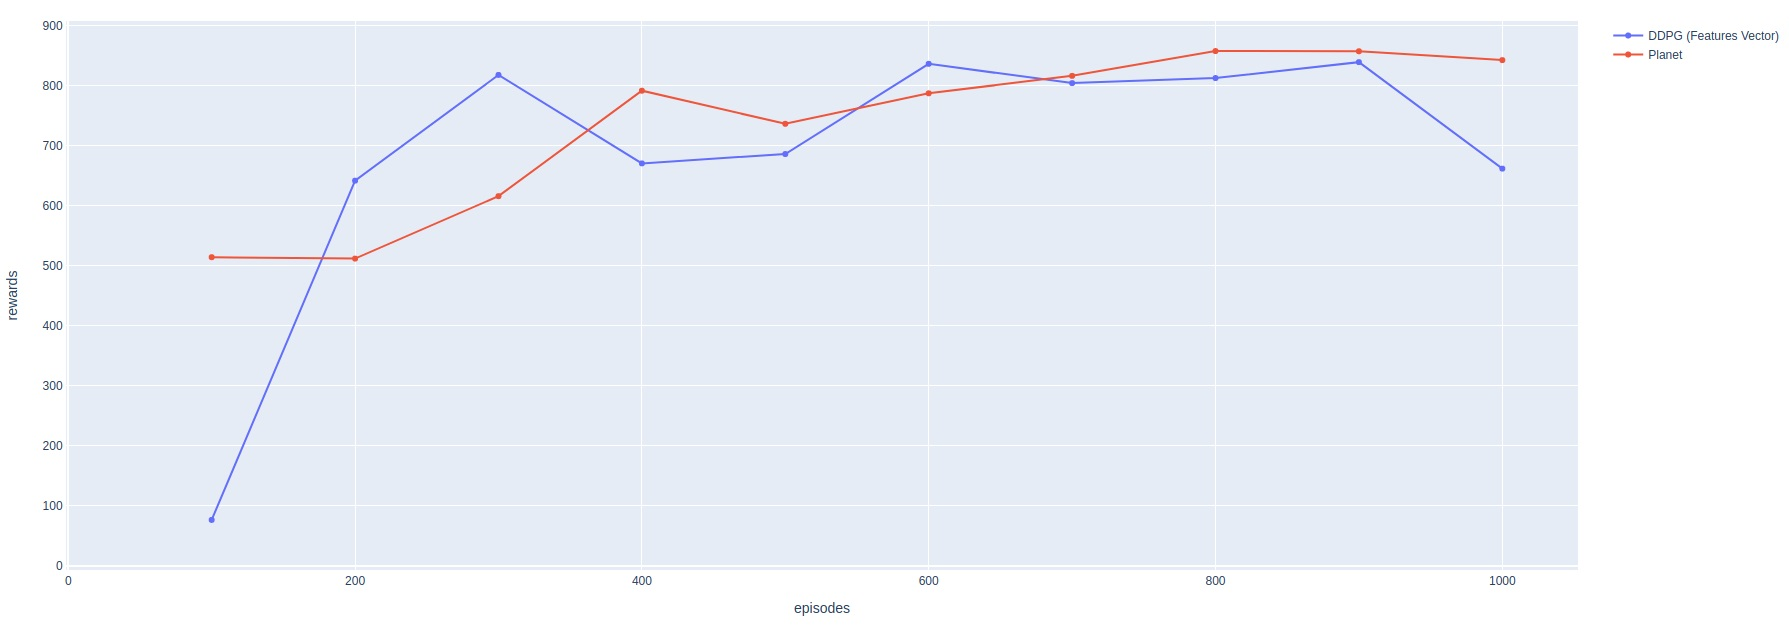
\includegraphics[width=1 \textwidth, height=.25\textheight]{pictures/cartpole_planet_vs_ddpg}
\caption{ Comparison between the performance of PlaNet (trained from frames) and DDPG (trained fro features vectors) for the Cartpole-Swingup environment.  }
\end{figure}
\begin{figure}[H]
\centering
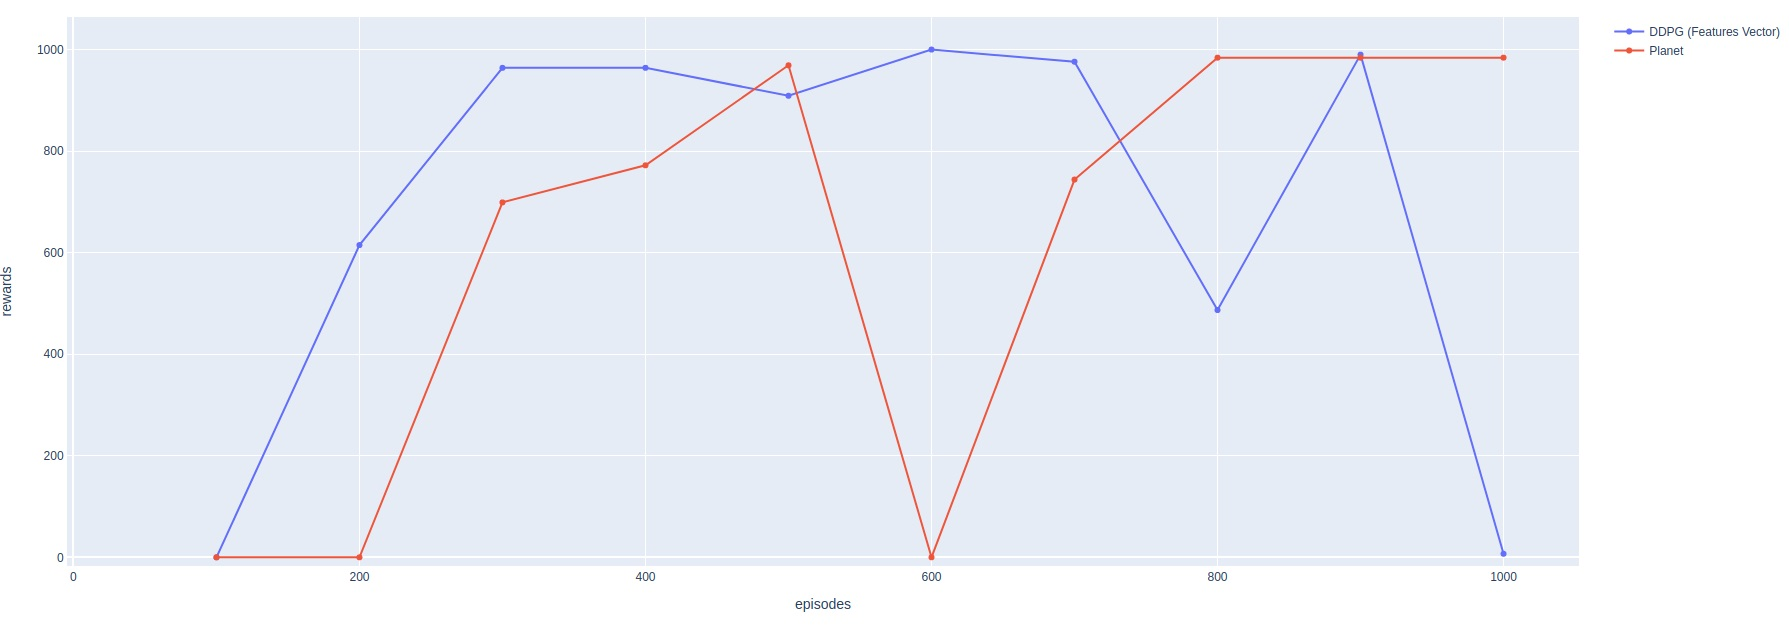
\includegraphics[width=1 \textwidth, height=.25\textheight]{pictures/reacher_planet_vs_ddpg}
\caption{ Comparison between the performance of PlaNet (trained from frames) and DDPG (trained fro features vectors) for the Reacher-easy environment.  }
\end{figure}
\begin{figure}[H]
\centering
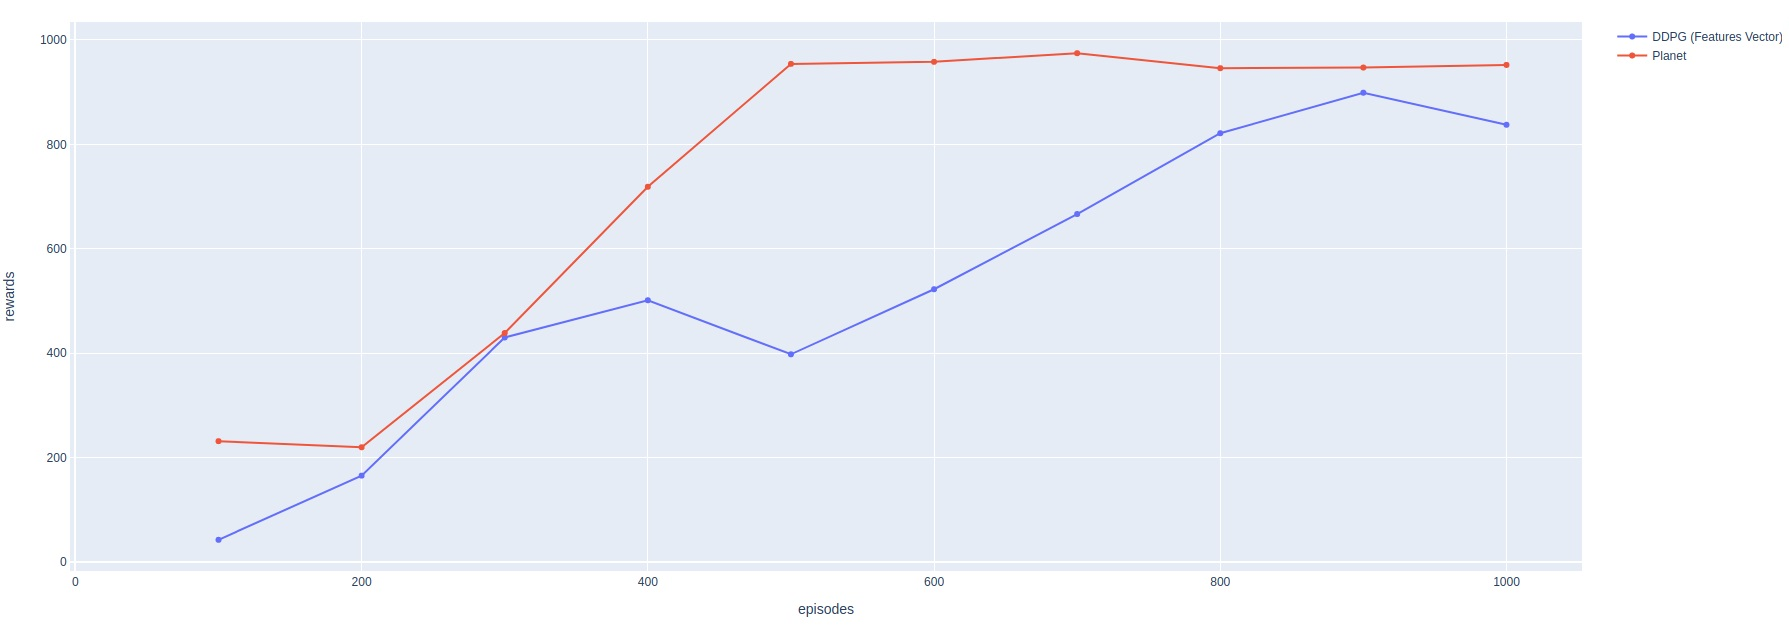
\includegraphics[width=1 \textwidth, height=.25\textheight]{pictures/walker_planet_vs_ddpg}
\caption{ Comparison between the performance of PlaNet (trained from frames) and DDPG (trained fro features vectors) for the Walker-walk environment.  }
\end{figure}

Coherently with the theory, we notice an evident difference between the training time for the model-based and model-free algorithm.
The PlaNet model can achieve a better result with less sample because it makes more calculations for each step. For this reason, the training time is longer when we train a model-based agent (the same is for the amount of GPU memory). Since the model-free has not a planner, it is also faster at inference time. 

\begin{figure}[H]
\centering
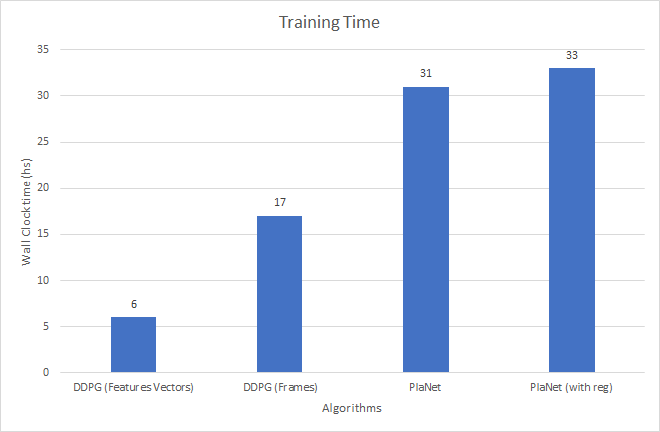
\includegraphics[width=1 \textwidth, height=.35 \textheight]{pictures/tempi_di_training}
\caption{ The plot shows a comparison between the training clock time (hours) required to train a DDPG linear model, DDPG convolutional model, PlaNet model and PlaNet model with the regularizer on a GPU Nvidia GeForce 1080ti..  }
\end{figure}